\chapter{Aspectos relevantes del desarrollo del proyecto}
\label{chap:desarrollo}

En este capítulo se expone la crónica del desarrollo de este TFG. Lejos de ser un proceso lineal, el trabajo ha seguido un camino iterativo, marcado por la investigación, la implementación de prototipos, la aparición de desafíos técnicos y la toma de decisiones estratégicas para superar los bloqueos. Esta narrativa busca reflejar fielmente el proceso de ingeniería real que he llevado a cabo, detallando no solo los éxitos, sino también los problemas y el proceso de depuración que ha sido necesario para resolverlos.

\section{Fase Inicial: Diseño de la Arquitectura y Selección de Tecnologías}
El proyecto comenzó con una fase de investigación y planificación, documentada en el Anexo apéndice:plan de proyecto. Durante esta etapa, se tomaron decisiones fundamentales sobre la pila tecnológica y el alcance inicial del proyecto.

\subsection{Selección de la Pila Tecnológica}
Basándome en los requisitos de construir un sistema de procesamiento de vídeo escalable, se realizo un estudio de las tecnologías de Big Data más adecuadas, como se detalla en el Capítulo \ref{chap:tecnicas_herramientas}. La pila tecnológica seleccionada fue:
\begin{itemize}
    \item \textbf{Jitsi/Jibri:} Como solución de código abierto para la captura de las sesiones de vídeo. Se ha optado por utilizar el proyecto oficial \texttt{docker-jitsi-meet} \cite{jitsi_docker_repo}, ya que proporciona una configuración pre-empaquetada con Docker Compose que, teóricamente, simplifica el despliegue de todos sus micro servicios (web, prosody, jicofo, jvb, jibri).
    \item \textbf{Apache Kafka:} Como bus de mensajería para desacoplar la captura del procesamiento.
    \item \textbf{Apache Spark:} Como motor de procesamiento distribuido para el futuro análisis de los datos.
\end{itemize}

\subsection{Definición del Alcance: Enfoque \textit{Offline} como Primer Hito}
Desde el principio, se conocia la complejidad de un sistema de procesamiento en tiempo real. La integración de un flujo RTMP de Jibri con Kafka y Spark Streaming presenta desafíos técnicos significativos. Por ello, se tomo una decisión estratégica clave para mitigar riesgos: \textbf{priorizar un flujo de trabajo \textit{offline} como primer objetivo funcional}. En este enfoque, Jibri grabaría las sesiones en archivos MP4, que se almacenarían en un sistema de ficheros accesible para que Spark los procesara por lotes. Esto me permitió dividir el problema en fases manejables, asegurando la entrega de una prueba de concepto funcional antes de abordar la complejidad del streaming en tiempo real.

\section{Fase I: El Desafío de Windows con WSL2}
\label{sec:desarrollo_acto1}
El primer intento de despliegue se realizó sobre el sistema de desarrollo principal: un sistema Windows 11 con el Subsistema de Windows para Linux (WSL2) y Docker Desktop. Aunque este entorno es muy versátil, la interacción entre el sistema de archivos de Windows (NTFS) y los permisos de Linux dentro de los contenedores demostró ser la fuente de problemas complejos y bloqueantes.

\begin{figure}[H]
    \centering
    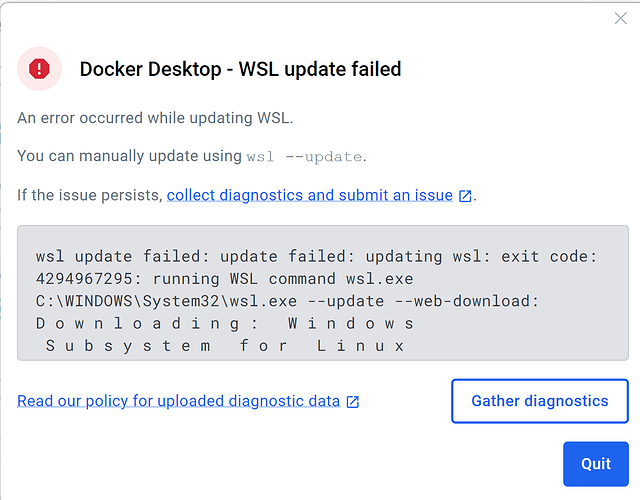
\includegraphics[width=\textwidth]{img/wsl2error.png}
    \caption{Ejemplo de algun error que surgio en esta fase wsl 2}
    \label{fig:Error WSL2}
\end{figure}

\subsection{Primer Despliegue de Jitsi y Análisis de Errores Críticos}
Tras clonar el repositorio de \texttt{docker-jitsi-meet} y configurar el fichero \texttt{.env}, el primer intento de levantar la pila de servicios con \texttt{docker-compose up} resultó en un fallo en cascada. Dos componentes clave, Prosody y Jibri, fallaban sistemáticamente.

\subsubsection{Errores de Permisos en el Contenedor Prosody}
El análisis de los \textit{logs} del contenedor de Prosody (el servidor XMPP) fue el primer indicio claro del problema subyacente. Los registros mostraban de forma repetida y consistente errores de tipo \texttt{"Permission denied"}, como se puede observar en este extracto:
\begin{verbatim}[frame=single, label={Fragmento de log de error de Prosody}]
datamanager error Unable to write to accounts storage 
('/config/data/auth%2elocalhost/accounts/focus.dat~:
Permission denied')
\end{verbatim}
Este error se debe a un conflicto en la gestión de permisos de ficheros entre sistemas operativos. El proceso de Prosody se ejecuta dentro del contenedor con un usuario y grupo específicos de Linux (\textit{uid/gid}), pero el volumen donde intenta escribir (\texttt{/config/data}) está montado desde el sistema de archivos NTFS de Windows a través de WSL2. La capa de traducción de permisos de WSL2 no era capaz de mapear correctamente los permisos, impidiendo que el proceso tuviera los privilegios de escritura necesarios. A pesar de intentar modificar los permisos en Windows y probar diferentes configuraciones de montaje de volúmenes en Docker, el problema persistió, indicando que se trataba de una limitación fundamental del entorno.

\subsubsection{Fallos de Autenticación en Cascada: Jibri y Jicofo}
El fallo de Prosody provocó un efecto dominó. \textbf{Jicofo}, el componente que gestiona las conferencias, no podía establecer conexión con el servidor XMPP. De forma aún más crítica, \textbf{Jibri}, el grabador de vídeo, fallaba con dos errores distintos:
\begin{itemize}
    \item Un error fatal \texttt{FATAL ERROR: Jibri recorder password and auth password must be set}, sugiriendo un problema en cómo se leían las variables de entorno desde el fichero \texttt{.env} en el entorno WSL2.
    \item Un error de autenticación: \texttt{SASLError using SCRAM-SHA-1:} \\
    \texttt{malformed-request}, consecuencia directa de no poder conectar con un servidor Prosody que no había logrado arrancar correctamente.
\end{itemize}

\subsection{Decisión Estratégica: Pivote a un Entorno Linux Nativo}
Tras un extenso periodo de depuración, se diagnosticó que los problemas de despliegue no residían en la configuración de Jitsi, sino en incompatibilidades fundamentales de la infraestructura de desarrollo basada en \textit{Windows} y \textit{WSL2}. La resolución de estos conflictos de bajo nivel, relacionados con la gestión de permisos y redes, se consideró un riesgo que desviaba el foco de los objetivos principales del proyecto.

En consecuencia, se tomó la decisión estratégica de migrar el entorno de desarrollo a un sistema operativo \textit{Linux} nativo. Se seleccionó \textit{Debian} debido a su reconocida estabilidad en entornos de servidor y su capacidad para proporcionar un entorno de ejecución predecible, eliminando las capas de compatibilidad que originaban los errores.

\section{Fase II: Implementación en Debian}
\label{sec:desarrollo_acto2}
La migración a un entorno Linux nativo fue un punto de inflexión en el proyecto. Como esperaba, los problemas de permisos relacionados con WSL2 desaparecieron de inmediato. Al ejecutar el comando \texttt{docker-compose up -d} en el directorio de \texttt{docker-jitsi-meet} , los cinco contenedores principales (prosody, jicofo, jvb, web y jibri) lograron arrancar y mantenerse en ejecución, un hito que no había sido posible alcanzar anteriormente.

Sin embargo, el éxito inicial solo reveló la siguiente capa de desafíos. A pesar de que los servicios estaban activos, la interfaz web de Jitsi no era accesible, mostrando un error de \textit{"La conexión ha fallado"}. Esto dio comienzo a un nuevo e intensivo ciclo de depuración, esta vez centrado en la configuración de la red y los componentes internos de Jitsi.

% S:captura 
\subsection{Proceso de Depuración de la Conexión HTTP}
Para solucionar el problema de conexión, se realizo un proceso de diagnóstico sistemático, analizando los \textit{logs} de cada contenedor y el comportamiento de la aplicación web para aislar la causa raíz.

\subsubsection{Diagnóstico del Protocolo de Conexión (WSS)}
El primer hallazgo importante se obtuvo al inspeccionar la consola de desarrollador del navegador. Esto revelo que, a pesar de que la instancia estaba configurada para HTTP, el cliente web intentaba establecer una conexión segura mediante el protocolo WebSocket Secure (WSS). Esto fallaba porque el servidor no tenía configurado ningún certificado SSL/TLS. La solución pasaba por forzar al cliente a utilizar una conexión no segura.

\begin{figure}[H]
    \centering
    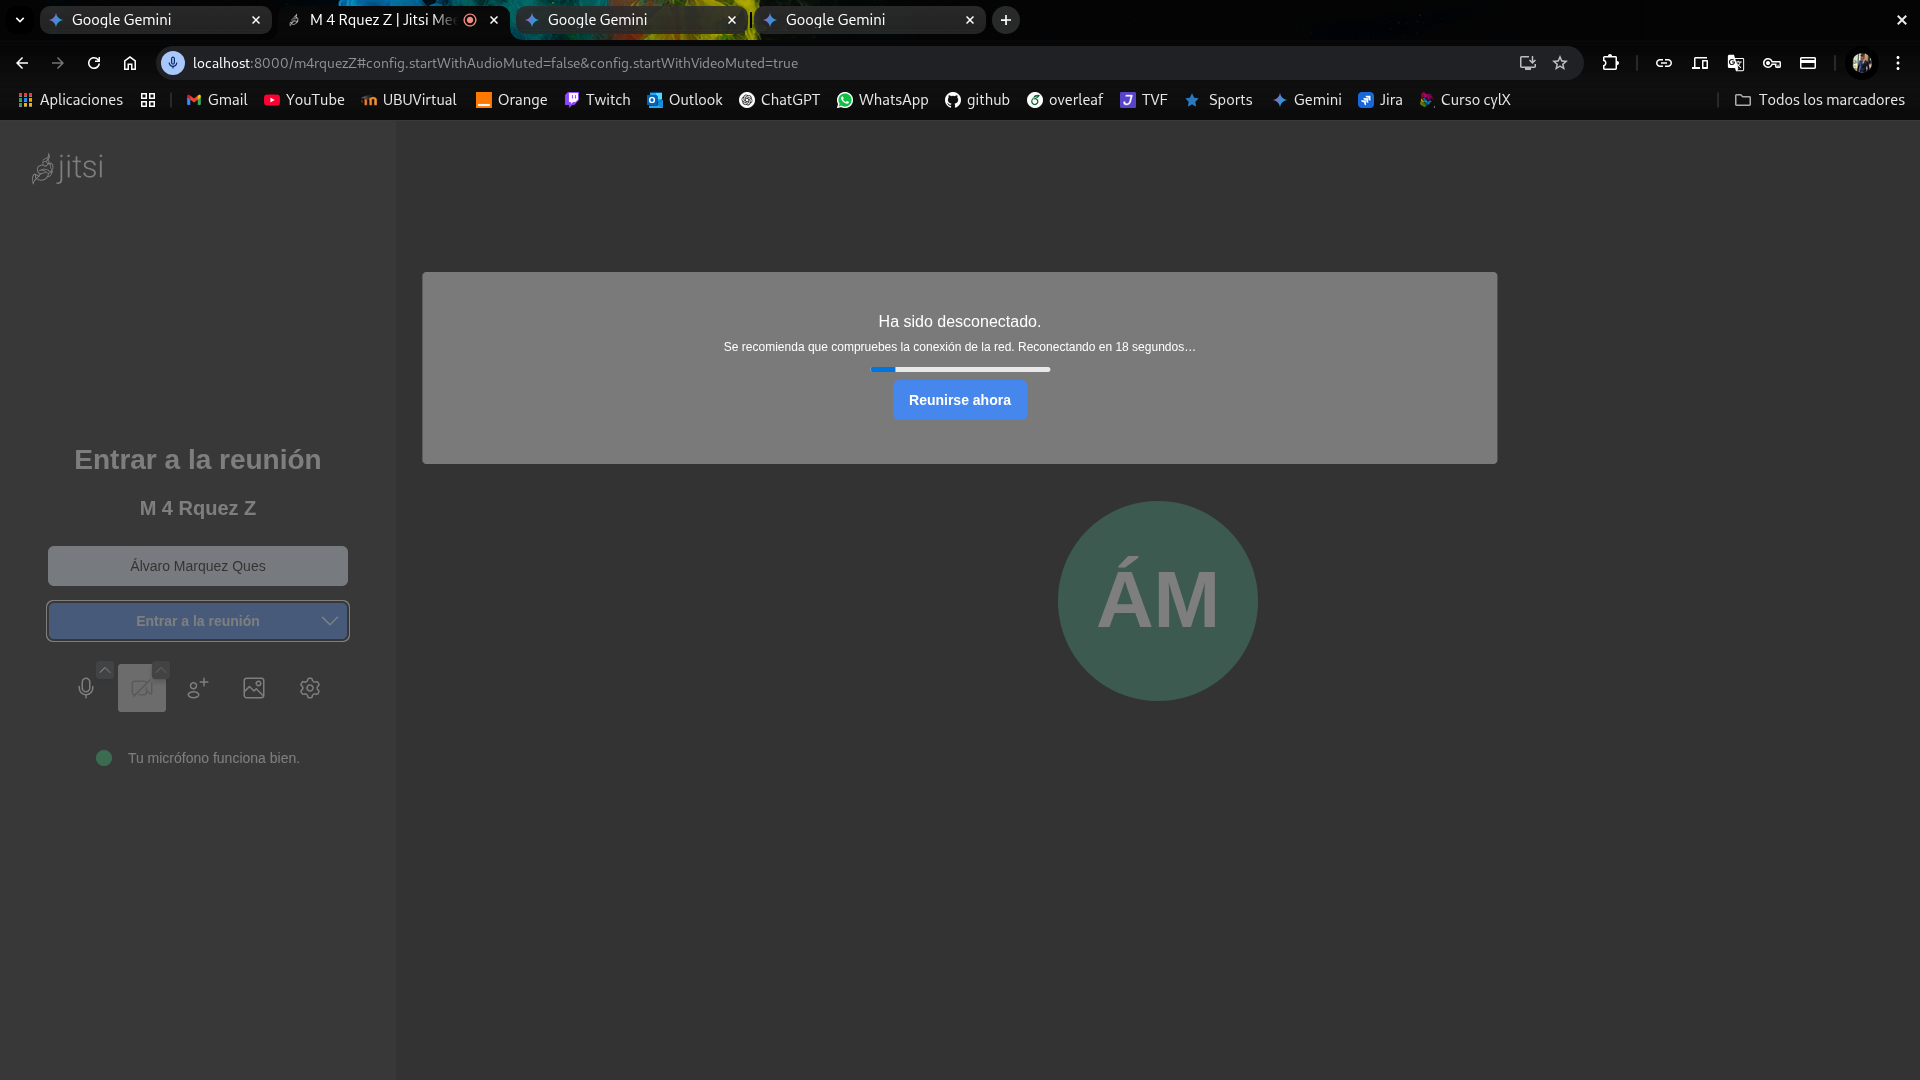
\includegraphics[width=0.8\textwidth]{img/errorconexion.png}
    \caption{Error de conexión inicial encontrado en el despliegue de Jitsi sobre Debian, a pesar de que los contenedores estaban en ejecución.}
    \label{fig:error_conexion_debian}
\end{figure}

\subsubsection{Solución y Error de Montaje: \texttt{custom.config.js}}
La documentación de Jitsi indica que se puede sobreescribir la configuración del cliente web mediante un archivo \texttt{custom.config.js}. Se decidió crear este archivo con el objetivo de deshabilitar la conexión segura. Sin embargo, al volver a lanzar los contenedores, el servicio web falló con un nuevo error: \texttt{...not a directory}. El problema era que Docker, al intentar montar el archivo de configuración en un volumen, se encontraba con que el directorio de destino ya había sido creado por el script de inicio del contenedor. La solución fue asegurar la creacion de la estructura de directorios y el fichero \texttt{custom.config.js} en la carpeta de configuración del host (\texttt{\textasciitilde{}/.jitsi-meet-cfg/web/}) antes de ejecutar \texttt{docker-compose up} por primera vez.

\subsubsection{Autenticación de Usuarios Anónimos (Invitados)}
Una vez solucionado el problema anterior, se logro acceder a la interfaz web, pero esto no hizo mas que generar un nuevo bloqueo: no se pudo crear una sala como usuario anónimo o invitado. Los \textit{logs} de Prosody indicaron que la autenticación para el dominio de invitados no estaba configurada. Para solucionarlo, se decicio que editar manualmente el fichero de configuración principal de Prosody (\texttt{prosody.cfg.lua}) y añadir un nuevo \texttt{VirtualHost} para \texttt{"guest.jitsi.localhost"}, habilitando explícitamente la autenticación anónima. Tras este cambio, finalmente se consiguio crear una conferencia y establecer una comunicación de vídeo y audio funcional.

\subsection{Iteración hacia HTTPS y Estrategia Actual}
Con el sistema funcionando en HTTP, y siguiendo las recomendaciones de los tutores, el siguiente paso fue intentar una implementación con HTTPS.
\begin{itemize}
    \item \textbf{Intento con Certificados Autofirmados:} El primer enfoque fue utilizar certificados autofirmados generados con la herramienta \texttt{mkcert}. Sin embargo, esto genero retroceder a un problema similar al de WSL2: el contenedor web de Jitsi (Nginx) no era capaz de leer o utilizar correctamente los certificados montados, provocando errores de SSL en el navegador.
    
    \item \textbf{Diagnóstico con OpenSSL:} Para diagnosticar el problema de forma precisa, se utilizo la herramienta de línea de comandos \texttt{openssl s\_client} para conectarme directamente al puerto 443 del servidor. El análisis confirmó que el servidor no estaba presentando el certificado que le había proporcionado, sino uno por defecto, lo que indicaba un fallo en la configuración de Nginx o en cómo Docker montaba los certificados. La herramienta \texttt{openssl s\_client} fue fundamental para este diagnóstico \cite{openssl_docs}.

    \begin{figure}[H]
    \centering
    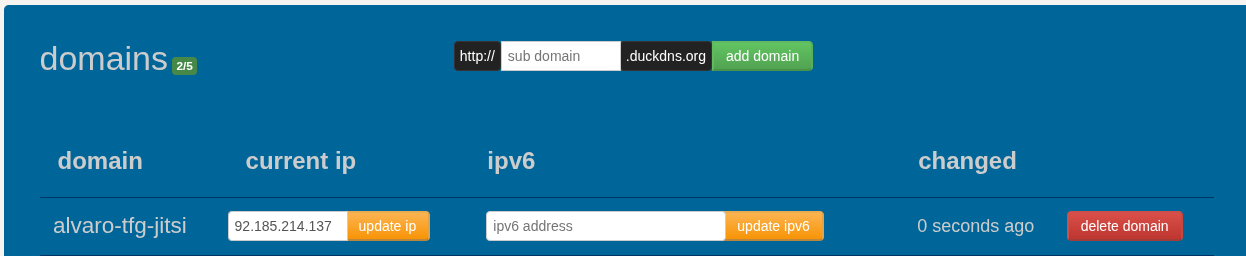
\includegraphics[width=0.9\textwidth]{img/duckdns.png}
    \caption{Panel de configuración de DuckDNS, donde se asocia un subdominio público a la dirección IP de la red local.}
    \label{fig:config_duckdns}
\end{figure}

\begin{figure}[H]
    \centering
    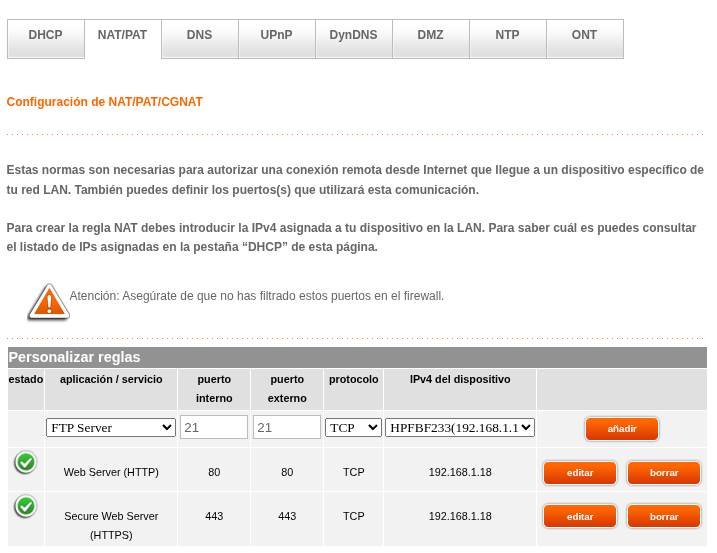
\includegraphics[width=0.9\textwidth]{img/routerconfig.png}
    \caption{Ejemplo de la configuración de redirección de puertos (Port Forwarding) necesaria para Jitsi y Let's Encrypt.}
    \label{fig:port_forwarding}
\end{figure}
    
    \item \textbf{Estrategia Definitiva (Let's Encrypt):} Basado en esta experiencia y en las indicaciones de los tutores, la estrategia actual y definitiva del proyecto es implementar HTTPS utilizando certificados válidos emitidos por una autoridad de certificación reconocida como \textbf{Let's Encrypt}. Este enfoque, aunque requiere un dominio público, garantiza una solución estándar, robusta y confiable, eliminando todos los problemas de confianza del navegador. Las tareas técnicas asociadas a esta implementación forman parte de la fase final del proyecto.
\end{itemize}

\begin{figure}[H]
    \centering
    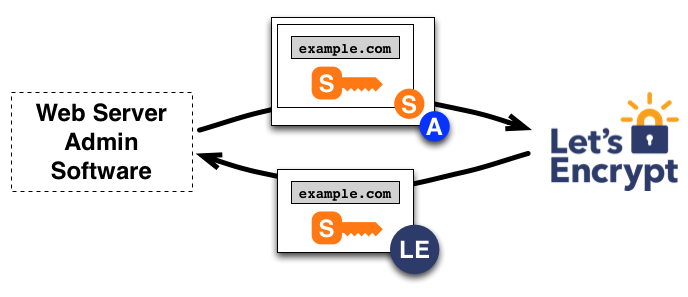
\includegraphics[width=0.9\textwidth]{img/letsencrypt.png}
    \caption{Ejemplo de funcionamiento Let's Encrypt.}
    \label{fig:Let's Encrypt}
\end{figure}

\section{Fase III: Consolidación de la Infraestructura}
\label{sec:desarrollo_acto_final}

Tras haber superado los problemas de conexión y configuración inicial en Debian, el proyecto entró en su fase final de implementación, cuyo objetivo era estabilizar por completo la infraestructura de Jitsi y desplegar y validar el pipeline de procesamiento de datos de extremo a extremo.

\subsection{Implementación de HTTPS con Let's Encrypt}
La estrategia de utilizar certificados autofirmados se demostró inviable. Por ello, se procedió a implementar la solución definitiva y robusta: la generación de certificados válidos mediante \textbf{Let's Encrypt}. El soporte nativo del proyecto \texttt{docker-jitsi-meet} para esta funcionalidad simplificó el proceso, aunque requirió una configuración cuidadosa del entorno de red:

\begin{itemize}
    \item \textbf{Dominio Público con DNS Dinámico:} Para que los servidores de Let's Encrypt pudieran verificar la propiedad del dominio, se utilizó un servicio de DNS Dinámico (\textbf{DuckDNS}). Este servicio proporcionó un subdominio público gratuito que se configuró para apuntar a la dirección IP pública de la red donde residía el servidor de desarrollo.
    
    \item \textbf{Redirección de Puertos (\textit{Port Forwarding}):} Se configuró el \textit{router} para redirigir el tráfico de los puertos necesarios (TCP 80 y 443 para HTTPS, y UDP 10000 para el tráfico de medios) desde la IP pública hacia la IP privada de la máquina Debian.
\end{itemize}

Una vez configurado el entorno de red, bastó con habilitar las variables correspondientes en el fichero \texttt{.env} de Jitsi. Al levantar los contenedores, los \textit{logs} del servicio web mostraron el proceso exitoso de validación y obtención del certificado, resultando en una instancia de Jitsi plenamente funcional y accesible a través de HTTPS con un certificado de confianza.

\begin{figure}[H]
    \centering
    
\includegraphics[height=0.6\textheight]{img/entrarreunion.jpg}
    \caption{Captura de la sala de entrada a la reunión de Jitsi sin errores}
    \label{fig: Sala entrada reunion jitsi}
\end{figure}

\subsection{Resolución de Desafíos Finales en Jibri}
Con la plataforma Jitsi estable, se realizaron las primeras pruebas de grabación con Jibri, que revelaron dos problemas finales:
\begin{enumerate}
    \item \textbf{Pantalla Negra en las Grabaciones:} El problema más crítico fue que los vídeos generados por Jibri contenían el audio correcto, pero la imagen era una pantalla negra. Tras una investigación muy exhaustiva no se ha podido solucionar esta problemática por lo tanto se dejara como linea de trabajo futura y mejora del proyecto.
    
    \item \textbf{Conexión Local de Jibri:} Se observó que, aunque los clientes externos podían conectarse a Jitsi sin problemas, Jibri (que se conecta desde dentro de la red Docker) fallaba al resolver la dirección del servidor. Esto finalmente paso a ser normalizado ya que la propia maquina Debian funciona como servidor que permite la conexión de los distintos dispositivos externos y no necesariamente debe funcionar localmente, al menos esa no es la intención principal, también puede dejarse pendiente como linea de trabajo futura.
\end{enumerate}

\subsection{Despliegue y Validación del Pipeline de Procesamiento}
Con el sistema de captura de vídeo completamente funcional, el último paso fue desplegar los componentes de procesamiento y validar el flujo de datos de extremo a extremo.
\begin{itemize}
    \item \textbf{Implementación del \textit{Script} de Procesamiento:} Se desarrolló el \textit{script} final en PySpark (\texttt{main.py}), incorporando la lógica de procesamiento inteligente que se describió en la fase de diseño. Este \textit{script} es capaz de detectar los vídeos más antiguos en el directorio de entrada, procesarlos, mover los ficheros originales a una carpeta de archivado y evitar el reprocesamiento. Se resolvieron, además, conflictos de dependencias, como el de NumPy con OpenCV, fijando las versiones en un fichero \texttt{requirements.txt} que se instala durante la construcción de la imagen Docker.
    
    \item \textbf{Prueba de Concepto y Validación End-to-End:} Se realizó una prueba completa del sistema. Una sesión de vídeo fue grabada con Jitsi, y el archivo MP4 resultante fue colocado en el directorio \texttt{/data}. A continuación, se ejecutó el \textit{pipeline} de procesamiento. El análisis de los \textit{logs} de la aplicación demostró que el \textit{script} localizó el vídeo, lo procesó aplicando la transformación de inversión de color, guardó el nuevo vídeo en la carpeta \texttt{/data/processed} y finalmente archivó el vídeo original. Este exitoso resultado validó la arquitectura completa y el correcto funcionamiento de todos los componentes integrados.
\end{itemize}

\begin{figure}[H]
    \centering
    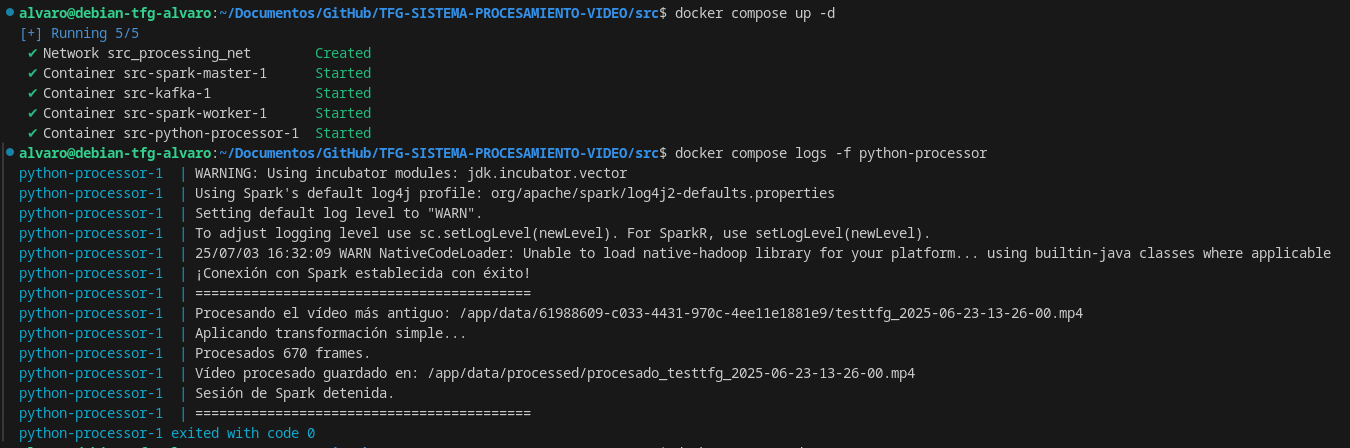
\includegraphics[width=\textwidth]{img/logsfinalpy.png}
    \caption{Captura donde se aprecia todos los contenedores funcionales y el script sin errores.}
    \label{fig:Logs Conexion completa sin errores}
\end{figure}

\begin{figure}[H]
    \centering
    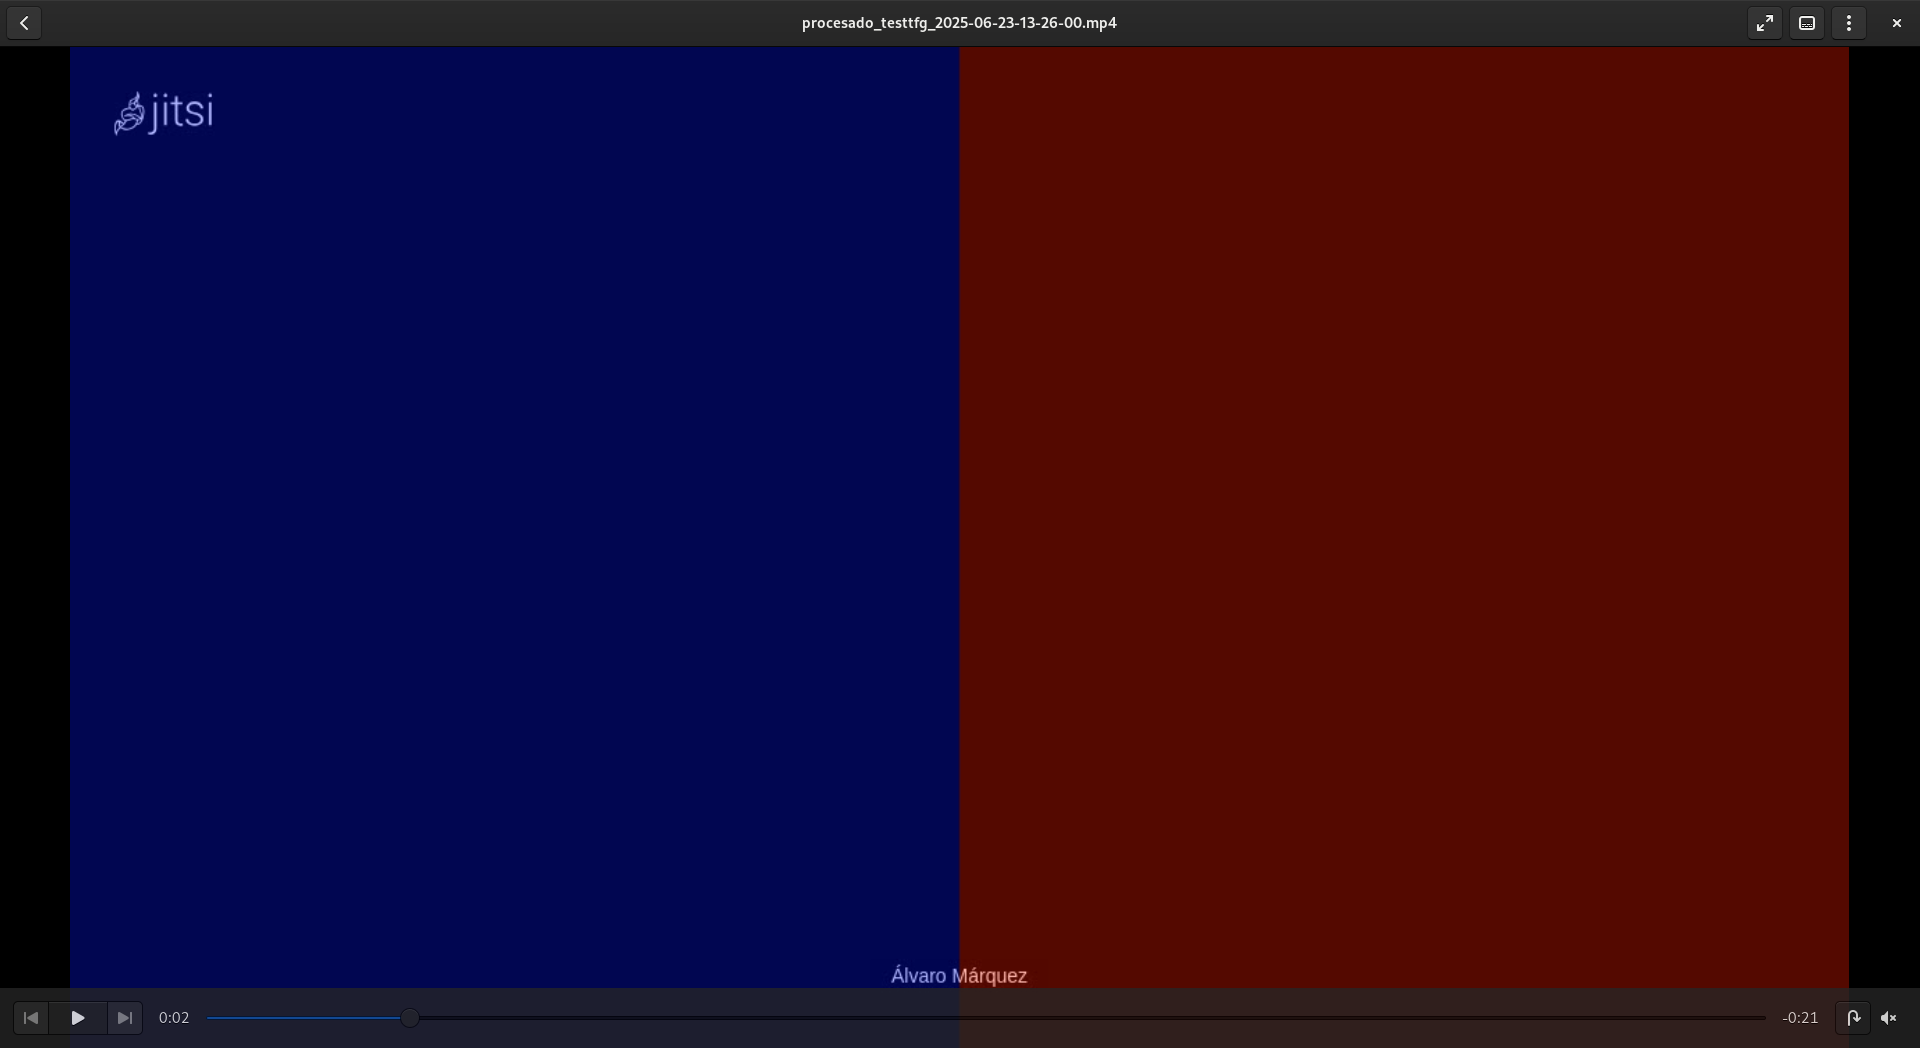
\includegraphics[width=\textwidth]{img/resultado-procesamiento.png}
    \caption{Captura donde se aprecia el video ya procesado mediante la transformación de color.}
    \label{fig:Captura video ya procesado}
\end{figure}

\subsection{Incorporación de Recursos Visuales}
Para mejorar la comprensión de la arquitectura y el flujo de trabajo descritos en este capítulo, se ha creado un conjunto de diagramas que se pueden encontrar en el Apéndice De Diseño. Estos recursos visuales incluyen un diagrama de la arquitectura general del sistema, un diagrama del pipeline de datos y un diagrama de despliegue de los contenedores Docker, entre otros. Estos elementos son fundamentales para clarificar las complejas interacciones entre los distintos componentes del sistema.